\documentclass[../MasterThesis.tex]{subfiles}
\graphicspath{ {./assets/images/} }


%----------------------------------------------------------------------------
%----------------------------------------------------------------------------

\begin{document}
	
	
\newpage

\section{README} \label{appendix:readme}


\subsection{Accurate-Player-3} \label{appendix:readmeaccurateplayer}

The README-file of the Accurate-Player-3 code was referenced as~\cite{RM_Frontend} and is included for transparency in the following.

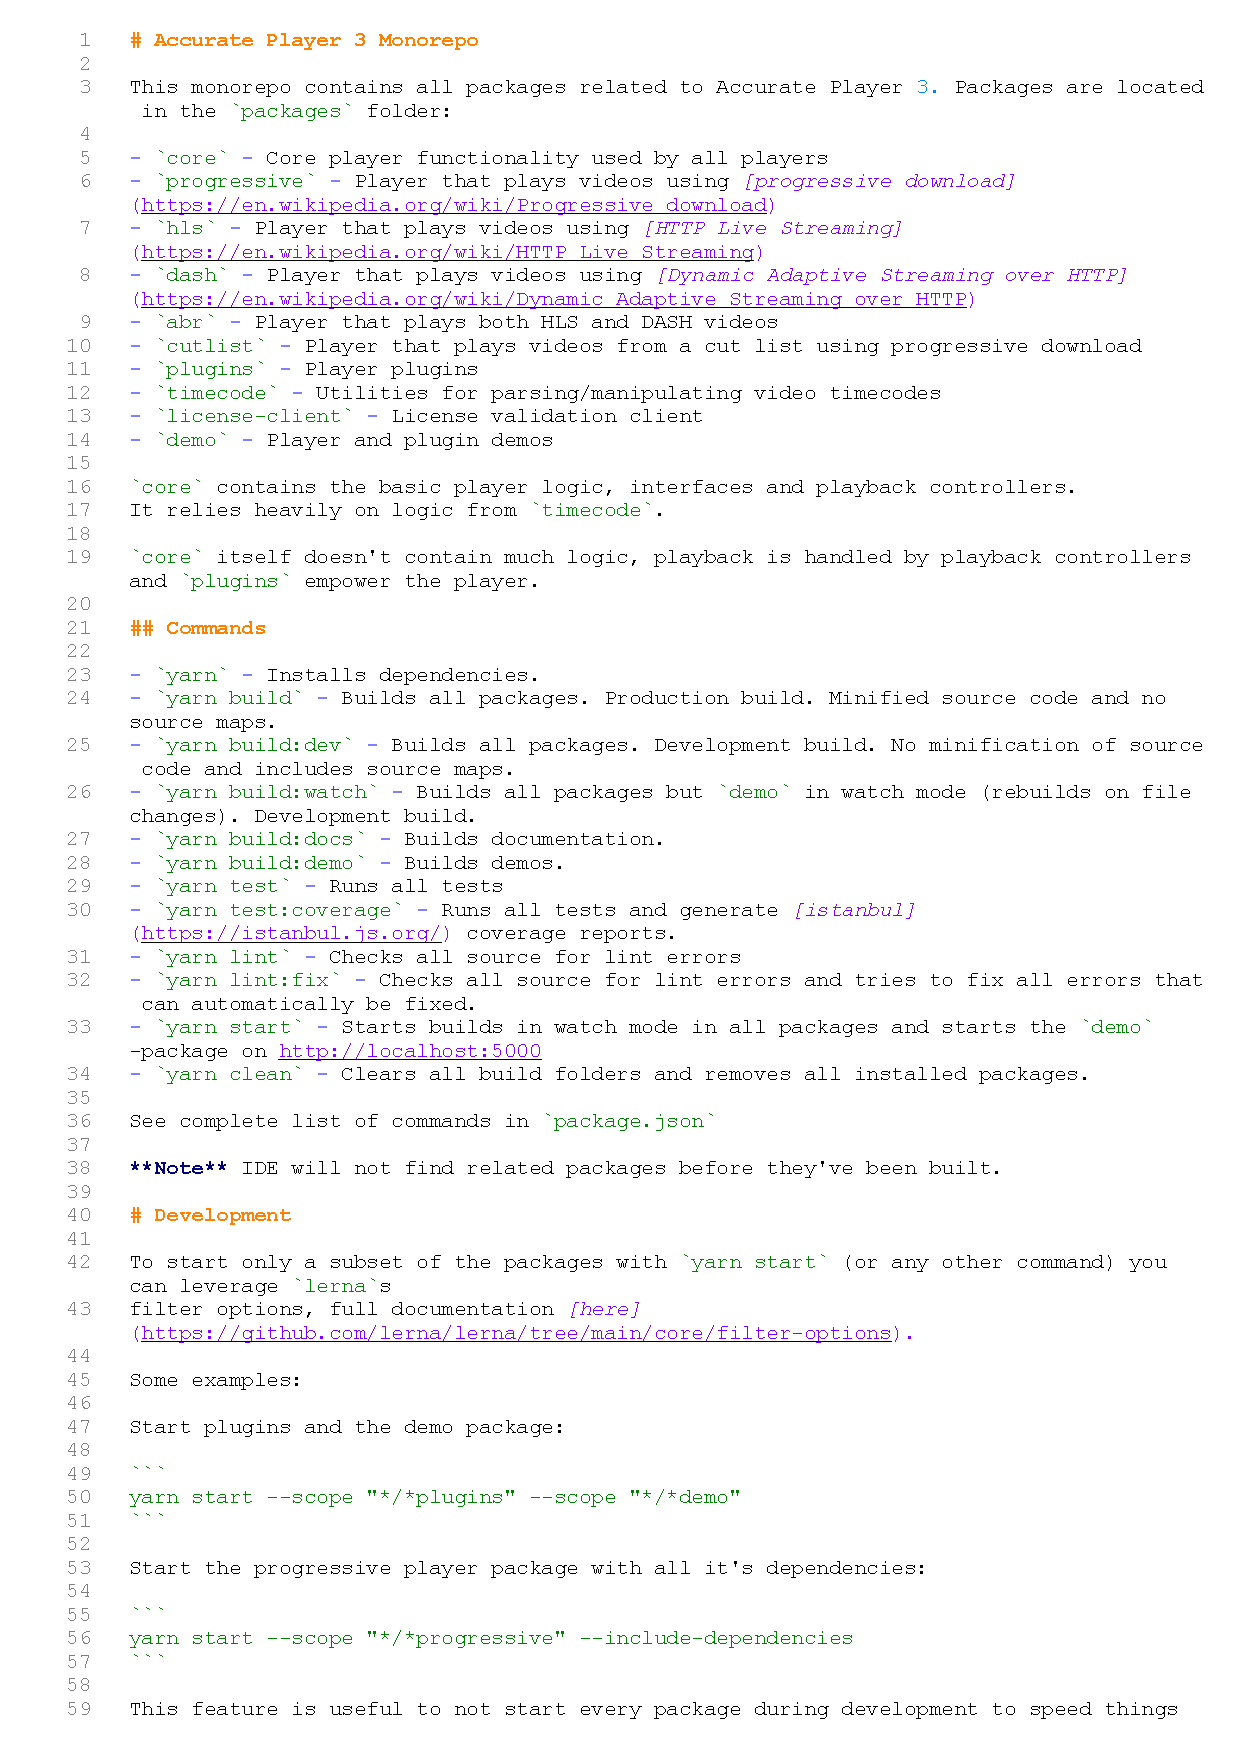
\includegraphics[page=1, width=0.9\textwidth]{FE.pdf}

\includegraphics[page=2, width=0.9\textwidth]{FE.pdf}



\newpage
\subsection{JIT-WebRTC} \label{appendix:readmejitwebrtc}

The README-file of the JIT-WebRTC code was referenced as~\cite{RM_Backend} and is included for transparency in the following.

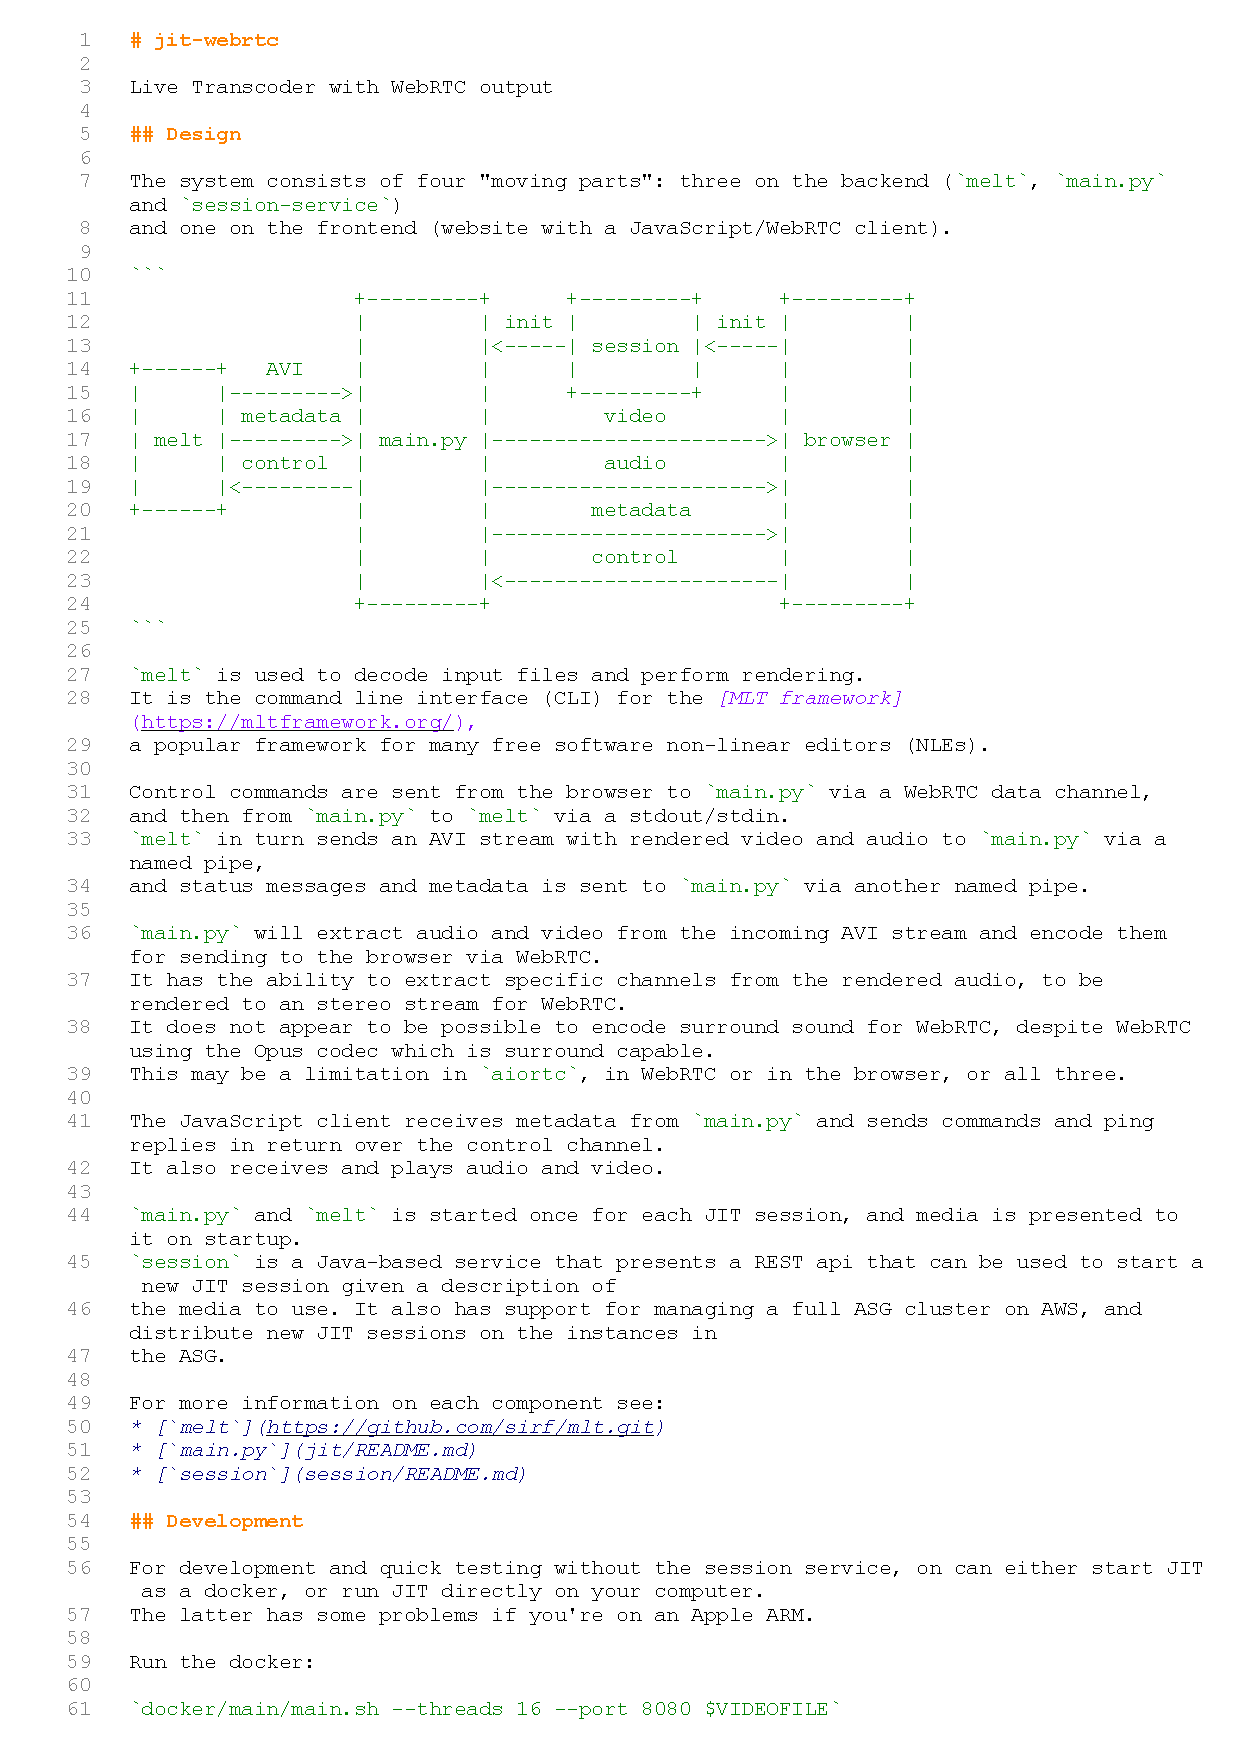
\includegraphics[page=1, width=0.9\textwidth]{BE.pdf}

\includegraphics[page=2, width=0.9\textwidth]{BE.pdf}


















%----------------------------------------------------------------------------
%----------------------------------------------------------------------------

\newpage
\section{Different Melt Filters} \label{appendix:differentMeltFilter}

In the following, different Melt filters, that influence the visual appearance of a video are listed. This list does not contain every filter and it the applied parameters for the different filter results vary. This is not a complete listing or analysis of the Melt filters but an overview over many of the filters and the options that arise from combining them or adapting the parameters. The complete list of filters without visual examples can be found on the Melt web site.~\cite{melt_filters}
%
\begin{figure}[H]
	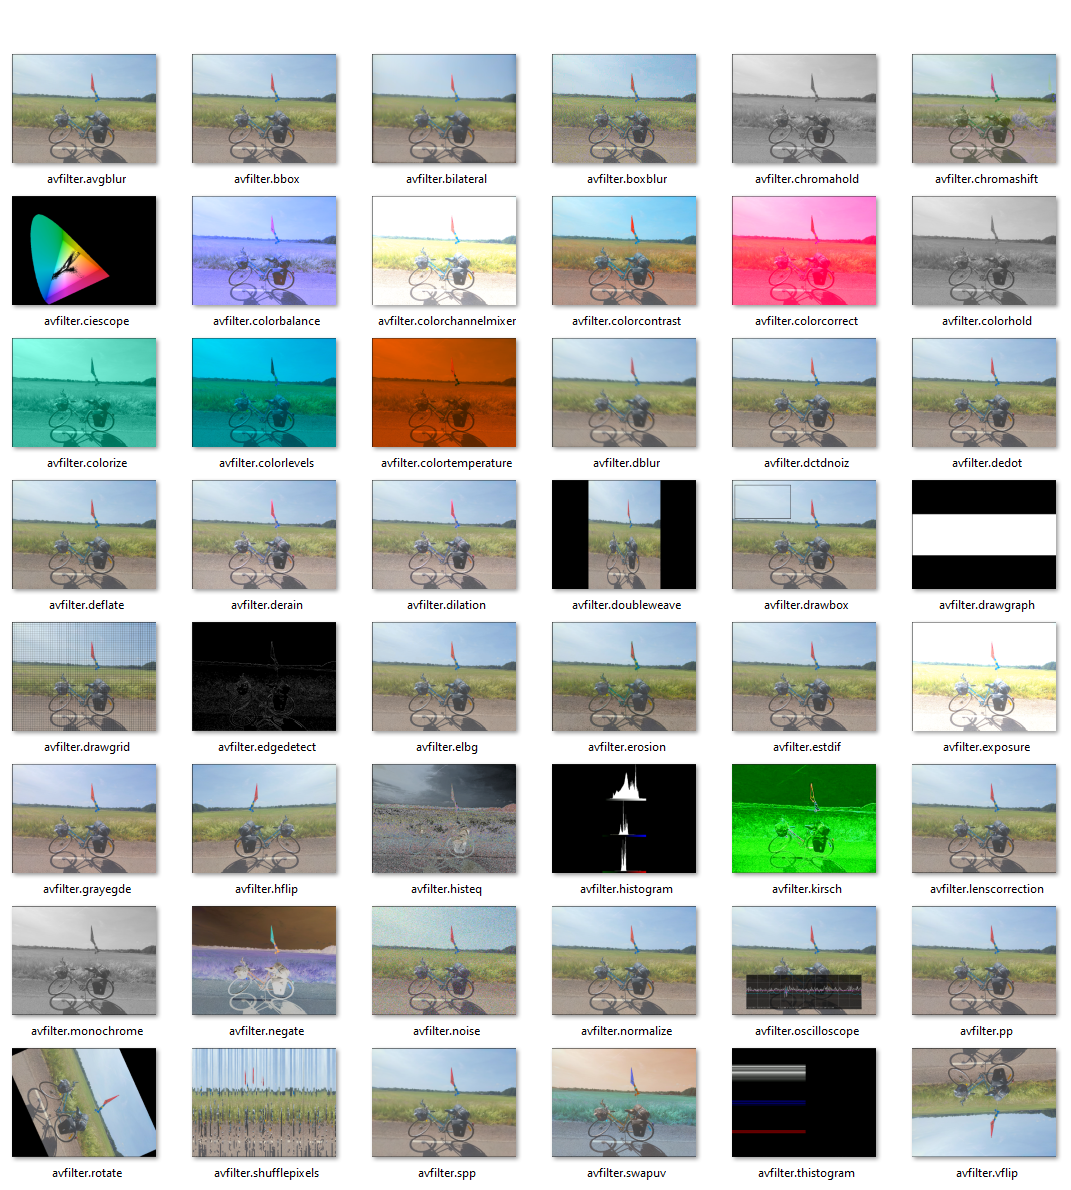
\includegraphics[width=1\textwidth]{Seite1.png}
\end{figure}

\begin{figure}[H]
	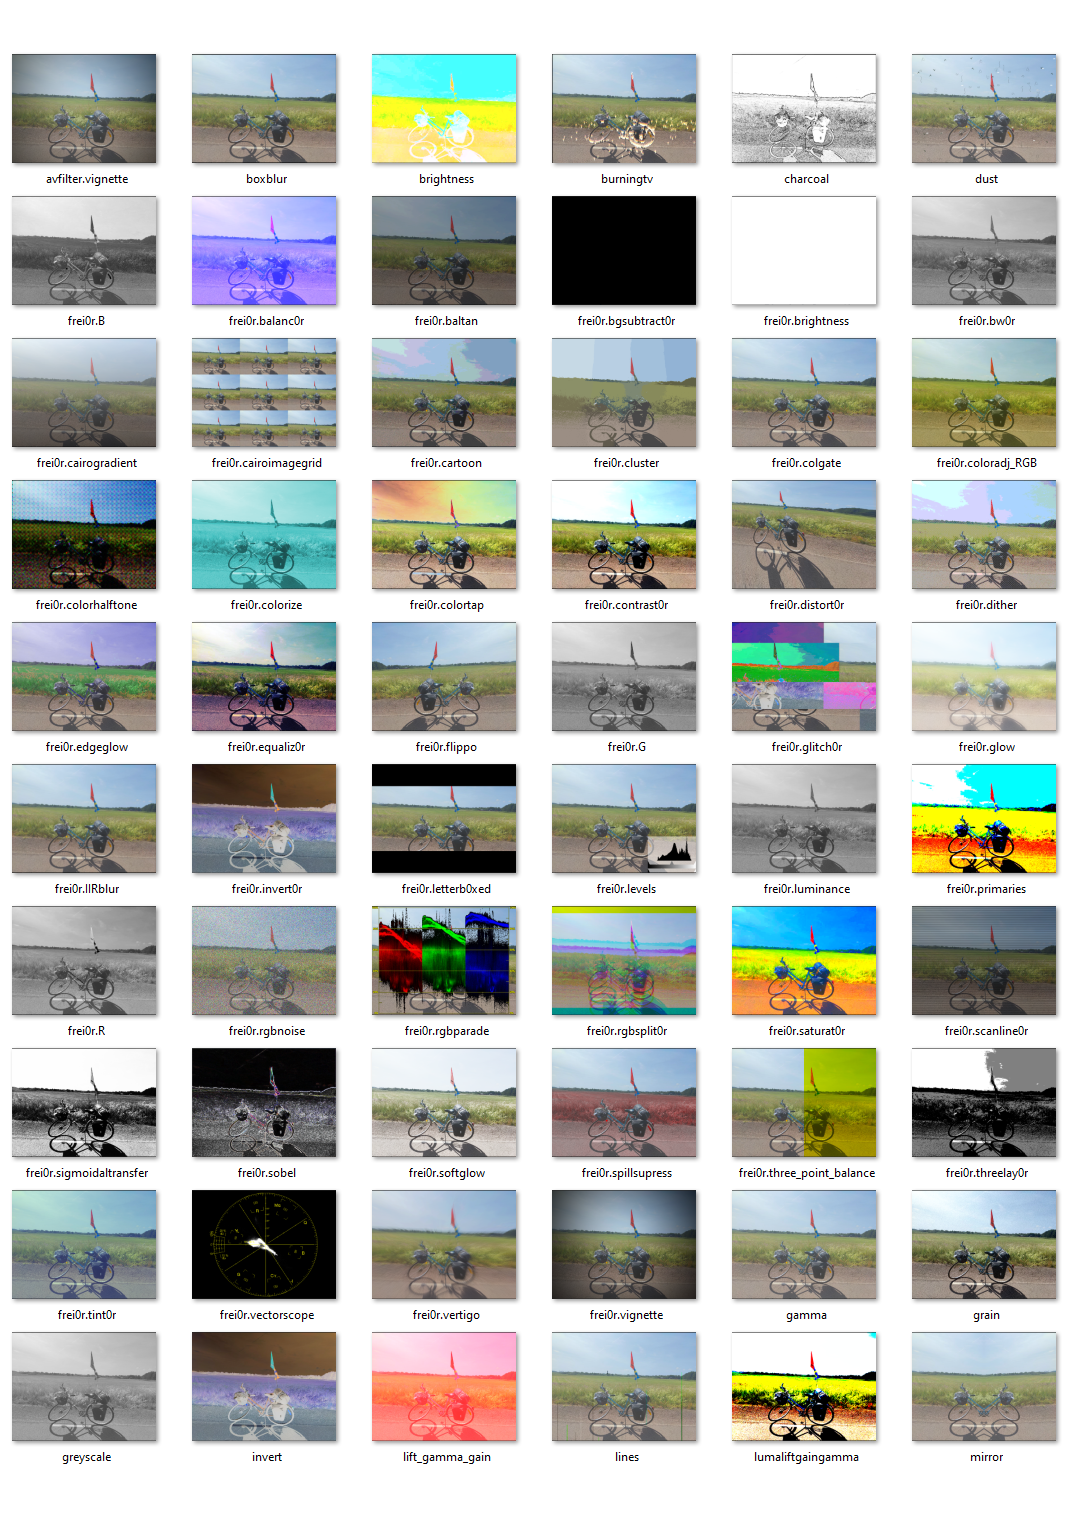
\includegraphics[width=1\textwidth]{Seite2.png}
\end{figure}

\begin{figure}[H]
	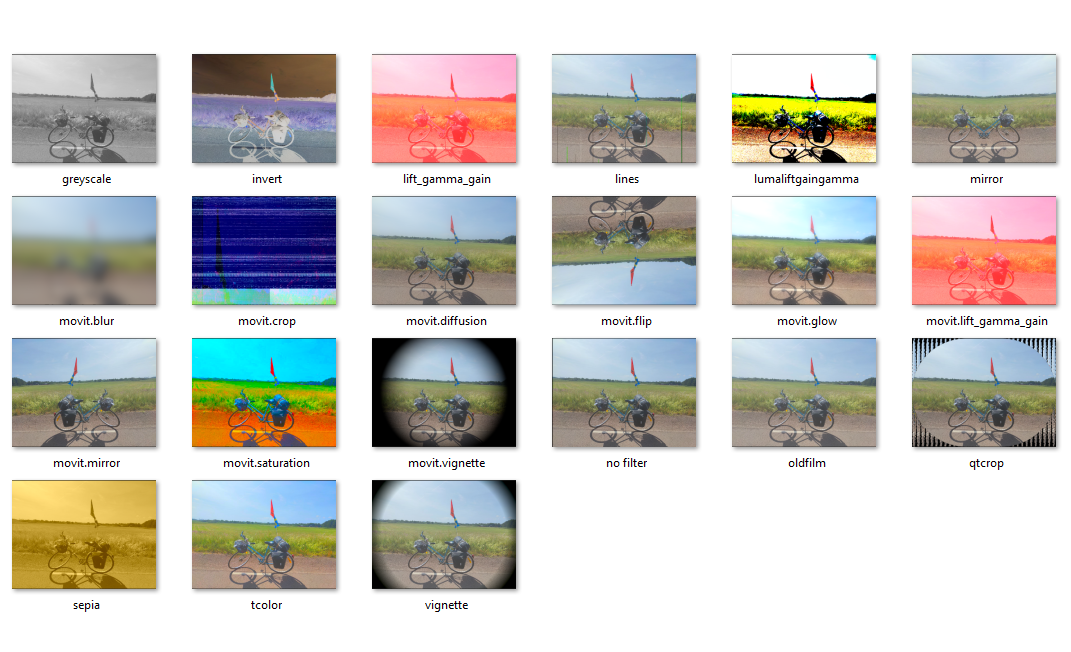
\includegraphics[width=1\textwidth]{Seite3.png}
\end{figure}







	
	
\end{document}